\documentclass[letter,11pt,oneside]{article}
%%% HEREHEREHERE
%%% APPENDIX
%%% ADDAPPENDIX
%%% (insert (format "\n%s\n" (buffer-file-name)))
%%% (occur "\\(\\\\[a-z]*section\\|appendix\\|input\\|\\<include\\>\\)")

%%\documentclass[11pt,twocolumn]{article}
%%\usepackage[inline]{asymptote}       %% Inline asymptote diagrams
%%\usepackage{wglatex}                 %% Use this one and kill others.
\usepackage{color}                     %% colored letters {\color{red}{{text}}
\usepackage{fancyhdr}                  %% headers/footers
\usepackage{fancyvrb}                  %% headers/footers
\usepackage{datetime}                  %% pick up tex date time 
\usepackage{lastpage}                  %% support page of ...lastpage
\usepackage{times}                     %% native times roman fonts
\usepackage{textcomp}                  %% trademark
\usepackage{amssymb,amsmath}           %% greek alphabet
\usepackage{parskip}                   %% blank lines between paragraphs, no indent
\usepackage{shortvrb}                  %% short verb use for tables
\usepackage{lscape}                    %% landscape for tables.
\usepackage{longtable}                 %% permit tables to span pages wg-longtable
\usepackage{multicol}                  %% Enhance footnotes/endnotes
\usepackage{url}                       %% Make URLs uniform and links in PDFs
\usepackage{enumerate}                 %% Allow letters/decorations for enumerations
\usepackage{endnotes}                  %% Enhance footnotes/endnotes
\usepackage{listings}                  %% Make URLs uniform and links in PDFs
\pdfadjustspacing=1                    %% force LaTeX-like character spacing
%%\usepackage{geometry}                  %% allow margins to be relaxed
%%\usepackage{wrapfig}                 %% permit wrapping figures.
%%\usepackage{subfigure}               %% images side by side.
%%\geometry{margin=1in}                  %% Allow narrower margins etc.
\usepackage[T1]{fontenc}               %% Better Verbatim Font.
\renewcommand*\ttdefault{txtt}        %% 
\usepackage[colorlinks=true]{hyperref} %% Make huperlinks within a PDF
\usepackage{natbib}                    %% bibitems
\usepackage{upquote}                   %% make programmer's quoetes in verbatim sections.

%% include background image (wg-document-page-background) 

\usepackage{graphicx}            %% Include pictures into a document
%% (wg-texdoc-inserttikz)


\def\documentisdraft{NOTDRAFT}

%% (wg-texdoc-isdraft)
%% (wg-texdoc-insert-fancy-headers)

%\usepackage[bookmarks]{hyperref} %% Make huperlinks within a PDF
\usepackage{makeidx}             %% Make an index uncomment following line
\makeindex                       %%.. yeah this one, too. index{key} in text




\definecolor{verbcolor}{rgb}{0.6,0,0}
\definecolor{darkgreen}{rgb}{0,0.4,0}
\newcommand\debate[1]{\textcolor{darkgreen}{DEBATE: #1} \marginpar{\textcolor{red}{DEBATE} }}
\newcommand{\ltodo}[2]{\marginpar{\textcolor{red}{ACTION: #1}\endnote{#2}}}
\renewcommand{\thefigure}{\thesection-\arabic{figure}}
\newcommand{\menu}{\ensuremath{\;\rightarrow\;}}
\newcommand{\dhl}[1]{{\color{verbcolor}{\texttt#1}}}
\definecolor{wglightgreen}{rgb}{0.88, 0.58, 0.88}
\newcommand{\wgtextbox}[1]{\noindent\fcolorbox{darkgreen}{wglightgreen}{%
    \minipage[t]{\dimexpr0.80\linewidth-2\fboxsep-2\fboxrule\relax}
        {#1}
    \endminipage}}

\usepackage[listings,breakable]{tcolorbox}

% \snippet{Caption}{file with body}
\newcommand\snippet[2]{%
\begin{figure}
\begin{tcolorbox} [breakable,colback=yellow!99!black!20]
\begingroup \fontsize{10pt}{10pt}
\selectfont
\VerbatimInput{snippets/#2}    % INPUT THIS FILE
\endgroup
\end{tcolorbox}
\caption{#1}
\label{fig:KStarsPreliminary}
\end{figure}
}

\newcommand\inlinesnippet[1]{%
\begin{figure}
\begin{tcolorbox} [breakable,colback=yellow!99!black!20]
\begingroup \fontsize{10pt}{10pt}
\selectfont
\begingroup \fontsize{10pt}{10pt}
\selectfont
\begin{Verbatim} [commandchars=\\\{\}]
#1
\end{Verbatim}
\endgroup

\endgroup
\end{tcolorbox}
\caption{Install KStars and other handy programs.}
\label{fig:KStarsPreliminary}
\end{figure}
}


%%(wg-add-inline-images)  %% add inline images to the mix




%%Begin User Definitions: Hint: ~/.latex.defs and  latex.defs  
%%End User Definitions:

%% (wg-texdoc-adjust-paper-width)
%% (wg-texdoc-insert-hypersetup)
%% (wg-latex-tablet-page)
%%%%%%%%%%%%%%%%%%%%%%%%%%%%%%%%%%%%%%%%%%%%%%%%%%%%%%%%%%%%%%%%%%%%%%%%%%%%%
%%%%%%%%%%%%%%%%%%%%%%%%%%%      PAGE SIZE      %%%%%%%%%%%%%%%%%%%%%%%%%%%%%
%%%%%%%%%%%%%%%%%%%%%%%%%%%%%%%%%%%%%%%%%%%%%%%%%%%%%%%%%%%%%%%%%%%%%%%%%%%%%
%%%%%%%%%%%%%%%%%%%%%%% comment usepackage geometry above %%%%%%%%%%%%%%%%%%%
% \usepackage{fancyhdr}            %% headers/footers
% remove references to package geometry
\pagestyle{fancy}
\usepackage[paperheight=7.125in,paperwidth=9.5in,footskip=.05in,margin=.75in,heightrounded]{geometry}

% (iv (setq tmp (/ (* 3.0 9.5) 4.0 )))   7.125
\fancyhf{}
%\cfoot{{\tiny Page \thepage \hspace{1pt}}}




%%%%%%%%%%%%%%%%%%%%%%%%%%%%%%%%%%%%%%%%%%%%%%%%%%%%%%%%%%%%%%%%%%%%%%%%%%%%%


\begin{document}


%% (wg-latex-pretty-title-page)
%%%%%%%%%%%%%%%%%%%%%%%%%%%% START PRETTY TITLE PAGE %%%%%%%%%%%%%%%%%%%%%%%%%%%%%%%%%

\vskip 1.5cm



 {\Huge FlexBerry}


\begin{figure}[h!]
\centering
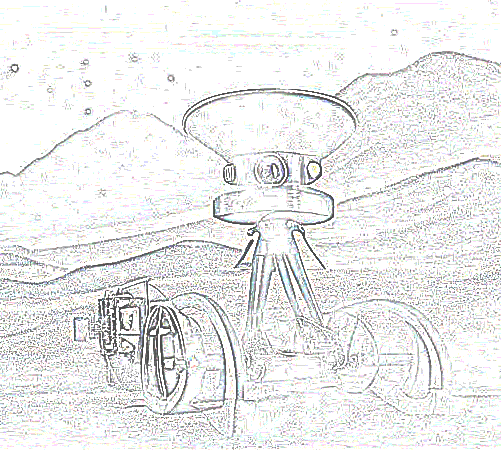
\includegraphics[width=.65\textwidth]{images/FlexBerry.png}\\
\hskip 4cm {\tiny AI art via nightcafe.studio for ``Spectrograph Telegraph Wonder''}
\end{figure}


%%%%%%%%%%%%%%%%%%%%%%%%%%%% END PRETTY TITLE PAGE %%%%%%%%%%%%%%%%%%%%%%%%%%%%%%%%%

%% (wg-texdoc-titleblock)
\pagenumbering{gobble}
\newpage
\section*{Preamble}

The cover art was generated at \url{https://images.nightcafe.studio/}
using the keywords ``Spectrograph Telegraph Wonder''. It was further
processed in a way to reduce toner use with Gimp. Presented here is
the AI Generated first cover art I've ever used for my notes!

\newpage

\title{FlexSpec1 Raspberry Pi Startup Guide}
\author{FS1 Team}
\date{\today}
\maketitle

\begin{abstract}
Acquire the latest image of Ubuntu 22.04 from Canonical for the
Raspberry Pi.  Burn the ISO image onto a high quality SD Card.  Start
the system and 'take the quiz': language, keyboard, geographic
location, user name and password, machine name etc.

Follow the \dhl{FollowMe.sh} script to do a full installation.

In this case, the user is \dhl{fred}, the machine runs DHCP and has
the name of \dhl{pier15}. See Section \ref{sec:Namesplaces}

\end{abstract}

%%%%%%%%%%%%%%%%%%%%%%%%%%%%%%%%%%%%%%%%%%%%%%%%%%%%%%%%%%%%%%%%%%%%%%%%%%%%%
%% table of contents
%%%%%%%%%%%%%%%%%%%%%%%%%%%%%%%%%%%%%%%%%%%%%%%%%%%%%%%%%%%%%%%%%%%%%%%%%%%%%
\pagenumbering{gobble}
\clearpage
\pagenumbering{roman}   % i,ii,etc
%%\pagenumbering{gobble}   %ignore page numbers for a while
\pdfbookmark[0]{Table of Contents}{MyTOC} % if usepackage{hyperref} in use.
\tableofcontents
\listoffigures
\listoftables
\newpage


\setcounter{section}{1}
\pagenumbering{arabic}

\ifx\documentisdraft\drafttest
\linenumbers    %%%%%%%%%%%%% DRAFT
\fi
\cfoot{{\tiny Page \thepage \hspace{1pt}}}

\section*{Overview}
\addcontentsline{toc}{section}{Overview}
\setcounter{page}{1}

This FlexBerry implementation uses Ubuntu 22.04 and NOT the Raspbian
image based on Ubuntu programs. The prescription for making this
system is contained in the GitHub repo TheSMTSci/FlexSpec1 repo. This
must be installed on the FlexBerry early on during its creation. This
document steps you through the install. See Section \ref{sec:raspbian}

This section builds the first working image, copy this image to an
iso file and make duplicate SD cards for use through out the system.
A small script to adjust each macnine's host name and IP address is
run for second/subsequent Raspberry Pis in the system.

The main script is situated at \dhl{\$HOME/git/FlexSpec1/code/HOME/FollowMe.sh}
in the git repository.

The basic steps:
\vspace{-.15cm}
\begin{enumerate}\addtolength{\itemsep}{-0.5\baselineskip}
%\setcounter{enumi}{N}
   \item   Get the Raspberry Imager if you don't have it.
   \item   Dwonload the Ubuntu 22.04 image.
   \item   Make the SD image.
   \item   Insert the SD into a Raspberry Pi 4b with attached Monitor/keyboard/mouse.
  This is needed to do a few very early steps.
   \item   Powerup/Boot the Raspberry Pi.
   \item   Take the usual Ubuntu quiz:\\
        username and password; machine name; country details etc.
   \item   The machine will reboot.
   \item   On the FlexBerry, open a terminal and start opening the new system up.
   \item   Download the rasp-config materials.
   \item   Run rasp-config and enable the serial port.
   \item   Now you get to reboot.
\end{enumerate}

Reboot with \dhl{sudo restart} command.

\snippet{Initial Commands. Bring install to current released content.}{01.txt}

\snippet{Add System User, get the FlexSpec1 git repository, run the script.}{02.txt}


The machine will be 'headless' -- meaning no keyboard/mouse/terminal
on the telescope. In order to communicate with the device, you will want
to start a ``ssh terminal session'' from the PC. This is standard with
Linux desktops, but needs additional packages for Win10/11 machines.

One of the best is PuTTY.

On your Windows machine, go to the Microsoft store and acquire PuTTY. Microsoft
perports this to be the safest way to install things on your machine.

\subsection{Cast of Characters}

Review the Scenario in Section \ref{Scenario} below.

For the local machine on a local lan,  assume:

\vspace{-.15cm}
\begin{enumerate}\addtolength{\itemsep}{-0.5\baselineskip}
%\setcounter{enumi}{N}
   \item   the Raspberry Pi is called \dhl{pier15}
   \item   We assume the default user's name is fred. (Note this is unique!)
   \item   It is found at \dhl{http://pier15.local}
   \item   It may be accessed with ssh: \\
  \dhl{ssh fred@pier15.local}
   \item   In addition to your login on the machine, we install a special user
  called \dhl{flex}. 
\vspace{-.15cm}
\begin{enumerate}\addtolength{\itemsep}{-0.5\baselineskip}
%\setcounter{enumi}{N}
   \item   The \dhl{flex} user holds all of our materials in its home directory.
   \item   These are critical to operation of FlexBerry.
\end{enumerate}
\end{enumerate}

Set Ubuntu's opinion of the  username for this machine. Here we use \dhl{pier15}.
Add the Country locale information, keyboard type, and we recommend
you think about boot without login.

At the console you want to add a few initial packages. The goal
is to use the \dhl{git} facility to download a copy of
\url{https://github.com/The-SMTSci/FlexSpec1} repository with
the comprehensive script of all the packages to load and configurations
to be made.


\section{The FlexBerry in action} \label{sec:FlexBerryInAction}

The FlexBerry has two main services running: the bokeh server for the GIU,
and a flexdispatch socket service to attach to the Arduino. These are
started and maintained by the OS and should not require any thought.
The FlexBerry runs the \dhl{nginx} web-server. This listens on port
80 -- per usual -- and offers access to documentation etc on each of
the FlexBerry Raspberry Pi machines. 




A special user \dhl{flex} will be added with a default password.

\vspace{-.15cm}
\begin{enumerate}\addtolength{\itemsep}{-0.5\baselineskip}
%\setcounter{enumi}{N}
   \item  Acquire the latest image of Ubuntu 22.04 from Canonical for the
Raspberry Pi.  

   \item  Burn the ISO image onto a high quality SD Card.

   \item  Insert the SD Card into the Pi and power on.

   \item  Start the system and 'take the quiz': language, keyboard, geographic
location, user name and password, machine name etc.
\end{enumerate}

\subsection{The Quiz} \label(sec:TheQuiz)

\dhl{The Quiz} consists of all the details a fresh Ubuntu system
needs to know. In particular is the user name and initial password.


A special user has been added: "flex". We recommend you keep this
user, as it retains some key "user level" data.

%%% HEREHEREHERE


\section{Scenario} \label{sec:Scenario}

The system is designed to run standalone without a router. It is
also designed to be part of a world-wide collaboration of like minded
sites; complete site with its domain name, subnets into observatories,
each observatory with its own subnet for one or more piers, each
pier with one or more OTAs; each OTA with one or more payloads.

The site's domain name:  example.com, with one observatory with
one telescope called \dhl{pier15}.

This  may be accessed at pier15.example.com in our scenario.

To make this happen DNS needs to be added to one Raspberry Pi within
the pier15 subnet. Instructions for this are included.

\section{Nginx Install}

We will add https to Nginx. This requires adding to \dhl{nginx.conf}

Nginx lives at \dhl{/etc/nginx}.

The pages for nginx lives at \dhl{/var/www/html} deep.

The HTML manual for the FlexSpec1 is at \dhl{http://pier15.local/flexhelp}.

The Arduino GUI is at \dhl{http://pier15.local/flexspec}. 


\subsection{Nginx Administration} \label{sec:NginxAdministration}

The \dhl{/etc/nginx/sites-available} has all the config information.

The \dhl{/etc/nginx/sites-enabled}   has the subset of files we're using.

Please don't mess around with this area unless you understand it, and need to.



\begingroup \fontsize{10pt}{10pt}
\selectfont
%%\begin{Verbatim} [commandchars=\\\{\}]
\begin{verbatim} 
TBD
\end{verbatim}
\endgroup
%% \end{Verbatim}



%%% APPENDIX
\appendix
\renewcommand \thesection{\Alph{section}}
\section{Names and Places} \label{sec:Namesplaces}

The design is one of using a network-enabled device on one of many
\dhl{piers} in an \dhl{observatory} at a \dhl{site}. There may be
one or more sites within a collaboration. One or more \dhl{collaborations}
within a \dhl{federation}\footnote{OK Too much late night Star Trek\copyright}.)

The observatory's Domain name will be referred to herein as the venerable
\url{https://example.com}. (Try it!) 

We assume multiple piers, each pier with one or more OTAs, each OTA with
one or more instruments under control of one or more Raspberry Pi's or
other hardware.

\section{Components of FlexBerry}

The \dhl{nginx} web engine is installed to provide the gateway to
the Bokeh code to communicate with the FlexSpec1's Arduino for motors,
etc. It also serves as the gateway to the interactive blog for observing
sessions. You may add additional pages to the \dhl{/var/www/html} section.

A bind9 DNS package is installed, and is used to provide subnet names
for the net behind the FlexBerry. There only should be one per subnet.
The bind9 package may be simple but it is often manages multi-site
corporate networks. We keep it simple.

In additon to nominal things installed as part of an Ubuntu 20.04 system,
we add the \dhl{supervisord} and \dhl{gunicorn} daemons to manage
flask/boheh web apps. This complexity permits access from outside the 
network.

\ltodo{Other Packages}{Explain other packages and subsytems.}

\newpage
\section{Certificates of Authority}

You can use a commercial Certifying Agency to manage \dhl{Certificates of Authority}
for you site/subnets or self-sign certificates. Here we play with self-signed certificates.
\index{Certificates of Authority}.

%\snippet{Self Signed Certificates}{ca1.txt}


\section{CertMe.sh}   \label{sec:CertMe}

This section covers issuing a 'self-signed-certificate' for nginx.
It is designed for local network use. We will enable ssh certificate
login AND keep PasswordAuthentication. PasswordAuthentication leaves
the machine open to brute force attacks -- we'll live with that for
now.

In order to ssh into the FlexBerry, adding a certificate mechanism
to the user's directory is not a bad or difficult thing to do.
Here are the steps. \index{Certificates of Authority!ssh}.

The files:

\begingroup \fontsize{10pt}{10pt}
\selectfont
%%\begin{Verbatim} [commandchars=\\\{\}]
\begin{verbatim} 
cd ~/.ssh
ssh-keygen
ssh-copy-id  wayne@pier15
\end{verbatim}
\endgroup
%% \end{Verbatim}


\snippet{Nginx Files}{certme1.txt}

%%% \begingroup \fontsize{10pt}{10pt}
%%% \selectfont
%%% %%\begin{Verbatim} [commandchars=\\\{\}]
%%% \begin{verbatim} 
%%% certs/
%%%    # nginx-selfsigned.crt dhparam.pem"
%%% openssl.cnf
%%% private/
%%%    # nginx-selfsigned.key  
%%% \end{verbatim}
%%% \endgroup
%%% %% \end{Verbatim}


\snippet{nginx sample file}{certme2.txt}

\section{Filesharing}

The FlexSpec, running on a Raspberry Pi, takes science images and may
store them locally in the Pi filesystem. It may also copy these files
to remote machine elsewhere. To work with file processing/viewing utilities
one has two choices:
\vspace{-.15cm}
\begin{enumerate}\addtolength{\itemsep}{-0.5\baselineskip}
%\setcounter{enumi}{N}
   \item   Move the file to the Remote machine, and use sofware there.
   \item   Install the package on the RPi
\end{enumerate}

Of the two, doint all processing/viewing on the remote machine makes the most
sense. This shifts the CPU load away from the instrumentation, and allows
programs native to a mix of operating systems to be used.

\subsection{NFS}



\begingroup \fontsize{10pt}{10pt}
\selectfont
%%\begin{Verbatim} [commandchars=\\\{\}]
\begin{verbatim} 
sudo apt install nfs-common
/mnt/share 10.0.0.0/24(rw,sync,no_subtree_check)
/export/flex 192.168.0.0/24(rw,async,no_subtree_check,anonuid=1000,anongid=1000)
sudo exportfs -a
sudo systemctl restart nfs-kernel-server
sudo ufw allow from 10.0.2.15/24 to any port nfs
sudo ufw enable
# sudo ufw status # look for 2049
\end{verbatim}
\endgroup
%% \end{Verbatim}



/subsection{SMB Windows Filesharing}

A SMB server is added to promote pushing image files to remote
servers during observing.

\begingroup \fontsize{10pt}{10pt}
\selectfont
%%\begin{Verbatim} [commandchars=\\\{\}]
\begin{verbatim} 
sudo apt install -y samba samba-tools smbclient cifs-utils
sudo systemctl enable --now smbd              # retister for all reboots
sudo ufw allow samba
sudo usermod -aG sambashare flex
sudo smbpasswd -a "flex%time has come"
sudo mkdir -p /samba/{$USER,flex}             # make shares for the two main users
sudo chgrp -R sambashare /samba
sudo usermod -aG sambashare $USER             # add these users to group
sudo usermod -aG sambashare flex
#smb://winhost/shared-folder-name
# TODO mod /etc/samba/smb.conf
sudo systemctl restart smbd
sudo systemctl restart nmbd
\end{verbatim}
\endgroup
%% \end{Verbatim}


Gnome's file manager has built in SMB support.

\url{https://wiki.samba.org/index.php/User_and_Group_management} has decent
examples.

/etc/samba/smb.conf:

   server role = standalone server
interfaces = 127.0.0.0/8 eth0
bind interfaces only = yes


[flex]
    path = /samba/flex
    browseable = no
    read only = no
    force create mode = 0660
    force directory mode = 2770
    valid users = flex @sadmin

\subsection{Flex Nginx Configuration}

This is a rambling collection of notes about the Nginx
install. This is initial setup:

\begingroup \fontsize{10pt}{10pt}
\selectfont
%%\begin{Verbatim} [commandchars=\\\{\}]
\begin{verbatim} 
FILE 50-mod-http-geoip2.conf
load_module modules/ngx_http_geoip2_module.so;
FILE 50-mod-http-image-filter.conf
load_module modules/ngx_http_image_filter_module.so;
FILE 50-mod-http-xslt-filter.conf
load_module modules/ngx_http_xslt_filter_module.so;
FILE 50-mod-mail.conf
load_module modules/ngx_mail_module.so;
FILE 50-mod-stream.conf
load_module modules/ngx_stream_module.so;
FILE 70-mod-stream-geoip2.conf
load_module modules/ngx_stream_geoip2_module.so;
\end{verbatim}
\endgroup
%% \end{Verbatim}



%%%ADDAPPENDIX

%% use a bibitem approach to the references publications etc.
%% (wg-bibitem)

%%\clearpage
\addcontentsline{toc}{section}{References}
\renewcommand*{\refname}{My Bibliography and References}
\bibliographystyle{apalike}	% bibliographystyle{apalike} and \usepackage{natbib}
\bibliography{MasterBib}	% expects file "MasterBib.bib"



%%\begin{thebibliography}{80}
%%\usepackage{natbib}   %% bibitems
%%\end{thebibliography}

%%\clearpage
\addcontentsline{toc}{section}{Index}
\printindex %% www.cs.usask.ca/resources/tutorials/latex/notes/toc-index.pdf

% /home/git/external/FlexSpec1/Code/rpi/tex/FollowMe.tex

%% (wg-texdoc-endnotes)

%%%%%%%%%%%%%%%%%%%%%%%%%%%%%%%%%%%%%%%%%%%%%%%%%%%%%%%%%%%%%%%%%%%%%%%%%%%%%
% Support for endnotes
\begingroup
\renewcommand{\notesname}{\textcolor{red} {Action Items:}}
\parindent 0pt
\parskip 2ex
\phantomsection
\addcontentsline{toc}{section}{	extcolor{red} {Action Items:}}
\def\enotesize{\normalsize}
\theendnotes
\endgroup

\end{document}

Ksk Royal -- basic install for Ubuntu 22.04
https://www.youtube.com/watch?v=YRgNcBdUHbo


